%
\documentclass[twoside]{article}
\setlength{\oddsidemargin}{0.25 in}
\setlength{\evensidemargin}{-0.25 in}
\setlength{\topmargin}{-0.6 in}
\setlength{\textwidth}{6.5 in}
\setlength{\textheight}{8.5 in}
\setlength{\headsep}{0.75 in}
\setlength{\parindent}{0 in}
\setlength{\parskip}{0.1 in}

%
% ADD PACKAGES here:
%

\usepackage{amsmath,amsfonts,graphicx}

%
% The following commands set up the lecnum (lecture number)
% counter and make various numbering schemes work relative
% to the lecture number.
%
\newcounter{lecnum}
\renewcommand{\thepage}{\thelecnum-\arabic{page}}
\renewcommand{\thesection}{\thelecnum.\arabic{section}}
\renewcommand{\theequation}{\thelecnum.\arabic{equation}}
\renewcommand{\thefigure}{\thelecnum.\arabic{figure}}
\renewcommand{\thetable}{\thelecnum.\arabic{table}}

%
% The following macro is used to generate the header.
%
\newcommand{\lecture}[4]{
   \pagestyle{myheadings}
   \thispagestyle{plain}
   \newpage
   \setcounter{lecnum}{#1}
   \setcounter{page}{1}
   \noindent
   \begin{center}
   \framebox{
      \vbox{\vspace{2mm}
    \hbox to 6.28in { {\bf EE502 - Linear Systems Theory II
	\hfill Spring 2023} }
       \vspace{4mm}
       \hbox to 6.28in { {\Large \hfill Lecture #1 \hfill} }
       \vspace{2mm}
       \hbox to 6.28in { {\it Lecturer: #2 \hfill } }
      \vspace{2mm}}
   }
   \end{center}
   \markboth{Lecture #1}{Lecture #1}

   \vspace*{4mm}
}
%
% Convention for citations is authors' initials followed by the year.
% For example, to cite a paper by Leighton and Maggs you would type
% \cite{LM89}, and to cite a paper by Strassen you would type \cite{S69}.
% (To avoid bibliography problems, for now we redefine the \cite command.)
% Also commands that create a suitable format for the reference list.
\renewcommand{\cite}[1]{[#1]}
\def\beginrefs{\begin{list}%
        {[\arabic{equation}]}{\usecounter{equation}
         \setlength{\leftmargin}{2.0truecm}\setlength{\labelsep}{0.4truecm}%
u         \setlength{\labelwidth}{1.6truecm}}}
\def\endrefs{\end{list}}
\def\bibentry#1{\item[\hbox{[#1]}]}

%Use this command for a figure; it puts a figure in wherever you want it.
%usage: \fig{NUMBER}{SPACE-IN-INCHES}{CAPTION}
\newcommand{\fig}[3]{
			\vspace{#2}
			\begin{center}
			Figure \thelecnum.#1:~#3
			\end{center}
	}
% Use these for theorems, lemmas, proofs, etc.
\newtheorem{theorem}{Theorem}[lecnum]
\newtheorem{lemma}[theorem]{Lemma}
\newtheorem{proposition}[theorem]{Proposition}
\newtheorem{claim}[theorem]{Claim}
\newtheorem{corollary}[theorem]{Corollary}
\newtheorem{definition}[theorem]{Definition}
\newenvironment{proof}{{\bf Proof:}}{\hfill\rule{2mm}{2mm}}

\newtheorem{exmp}[theorem]{Ex}

% **** IF YOU WANT TO DEFINE ADDITIONAL MACROS FOR YOURSELF, PUT THEM HERE:

\begin{document}

% Lecture Details
\lecture{4}{Asst. Prof. M. Mert Ankarali}



\section{Realization Theory}

\textbf{Definition:} A transfer function (matrix) $G(s)$ is said to be
realizable if there exist a (finite-dimensional) state-space
realization of it. 

\textbf{Theorem:} A Transfer-Function (matrix) $G(s)$ is realizable
$\Leftrightarrow$ $G_{ij}(s)$ is a proper rational transfer function
$\forall (i,j)$

\textbf{Proof:}

\textbf{Part I:} Show that $G(s)$ is realizable $\Rightarrow$
$G_{ij}(s)$ is proper $\forall (i,j)$

Assume $G(s)$ realizable $\exists  (A,B,C,D)$ tuple such that $G(s) =
C (sI - A)^{-1} B + D$

\begin{align*}
&\lim_{s \to \infty} G(s) = \lim_{s \to \infty}  \left[ C \left( s I -
  A \right)^{-1} B \right] = \lim_{s \to \infty}  \left[ \frac{ C \mathrm{Adj}\left( s
       I - A \right) B}{ \mathrm{Det}\left( s
       I - A \right) } + D \right] = D \ , \ where
\\
&| D_{ij} | < \infty \ \forall (i,j) \Rightarrow G_{ij}(s) \ \mathrm{is}
  \ \mathrm{proper} \ \forall (i,j)
\end{align*}

\textbf{Part II:} Show that $G_{ij}(s)$ is proper $\forall (i,j)$
$\Rightarrow$ $G(s)$ is realizable 

The task is to find $(A,B,C,D)$ tuple such that $G(s) = C (sI - A)^{-1} B + D$

\subsection{Canonical State-Space Realizations of SISO Systems}

For the sake of clarity, derivations are given for general $3^{rd}$ order LTI systems.

\subsubsection{CT Reachable/Controllable Canonical Form}

In this method of realization, we use the fact the system is
LTI. Let's consider the transfer function of the system and let's 
perform some LTI operations.
%
\begin{align*}
Y(s) &= \frac{ b_3 s^3 + b_2 s^2  + b_1 s + b_0 }{ s^3 + a_2 s^2 + a_1 s + a_0} U(s)
\\
&= \left( b_3 s^3 + b_2 s^2  + b_1 s + b_0 \right)  
\frac{1}{ s^3 + a_2 s^2 + a_1 s + a_0 } U(s) 
\\
&= G_2(s) G_1(s) U(s) \ \mathrm{where} 
\\
G_1(s) &= \frac{H(s)}{U(s)} = \frac{1}{ s^3 + a_2 s^2 + a_1 s + a_0 } 
\\
G_2(s) &= \frac{Y(z)}{H(z)} = b_3 s^3 + b_2 s^2  + b_1 s + b_0
\end{align*}
%
As you can see we introduced an intermediate variable $h(t)$ or with a
Laplace transform of $H(s)$. First transfer function has static input
dynamics, operates on $u(t)$, and produces an output, i.e. $h(t)$. 
Second transfer function is a ``non-causal'' system and operates on $h(t)$ and produces output
$y(t)$. If we write the ODEs of both systems we obtain
%
\begin{align*}
\dddot{h} &= -a_2 \ddot{h} - a_1 \dot{h} - a_0 h + u
\\
y &= b_3 \dddot{h} + b_2 \ddot{h} + b_1 \dot{h} + b_0 h
\end{align*}
%
Now let the state-variables be 
$x = \left[ \begin{array}{c} x_1 \\ x_2 \\ x_3 \end{array} \right] 
= \left[ \begin{array}{c} h \\ \dot{h} \\ \ddot{h} \end{array} \right]$. Then,
individual state equations take the form
%
\begin{align*}
\dot{x_1} &= x_2
\\
\dot{x_2} &= x_3
\\
\dot{x_3} &= -a_2 x_3 - a_1 x_2 - a_0 x_1 + u
\end{align*}
%
and the output equation take the form
%
\begin{align*}
y &= b_3\left( -a_2 x_3 - a_1 x_2 - a_0 x_1 + u \right) + b_2 x_3 +
    b_1 x_2 + b_0 x_1
\\
&= ( b_0 - b_3 a_0 ) x_1 + ( b_1 - b_3 a_1 ) x_2 + ( b_2 - b_3 a_2 ) x_3 + b_3 u
\end{align*}
%
If we re-write the equations in matrix form we obtain the state-space representation as
%
\begin{align*}
	\dot{x} &= \left[ \begin{array}{ccc} 0 & 1 & 0  \\  0 & 0 & 1 \\  -a_0 & -a_1 & -a_2 \end{array} \right] x 
	+ \left[ \begin{array}{c} 0 \\ 0 \\ 1 \end{array} \right] u
	\\
	y &= \left[ \begin{array}{ccc} ( b_0 - b_3 a_0 ) & ( b_1 - b_3 a_1 )  & ( b_2 - b_3 a_2 ) \end{array} \right] x
	+ \left[ b_3 \right] u
\end{align*}

If we obtain a state-space model from this approach, the form
will be in \textit{controllable canonical form}.  

For a general $n^{th}$ order transfer function controllable
canonical form has the following $A \ ,  B \ ,  C \ , \& \ D$
matrices

\begin{align*}
A &= \left[ \begin{array}{ccccc} 0 & 1 & 0 & \cdots & 0 \\ 0 & 0 & 1 &
                                                                      \cdots & 0
\\ \vdots & \vdots & \vdots & & \vdots
\\ 0 & 0 & 0 & \cdots & 1
    \\ -a_0 & -a_1 & -a_2 & \cdots & -a_{n-1} \end{array} \right]
\quad , \quad 
B = \left[ \begin{array}{c} 0\\ 0 \\ \vdots \\ 0
    \\ 1 \end{array} \right]
\\ C &= \left[ \begin{array}{cccc} (b_0 - b_n a_0) 
  &  (b_1 - b_n a_1) & \cdots & (b_{n-1} - b_n a_{n-1}) \end{array} \right]
\quad , \quad
D = b_n
\end{align*}

\subsubsection{DT Reachable/Controllable Canonical Form}

Similar to the CT case, we will use the fact the system is
LTI. Let's consider the transfer function of the system and let's 
perform some LTI operations.
%
\begin{align*}
Y(z) &= \frac{b_3 + b_2 z^{-1} + b_1 z^{-2} + b_0 z^{-3}}{1+ a_2
       z^{-1} + a_1 z^{-2} + a_0 z^{-3}} U(z)
\\
&= \left( b_3 + b_2 z^{-1} + b_1 z^{-2} + b_0 z^{-3} \right) \frac{1}{1+ a_2
       z^{-1} + a_1 z^{-2} + a_0 z^{-3}} X(z) 
\\
&= G_2(z) G_1(z) U(z) \ \mathrm{where} 
\\
G_1(z) &= \frac{H(z)}{U(z)} = \frac{1}{1+ a_2
       z^{-1} + a_1 z^{-2} + a_0 z^{-3}} 
\\
G_2(z) &= \frac{Y(z)}{H(z)} = b_3 + b_2 z^{-1} + b_1 z^{-2} + b_0 z^{-3} 
\end{align*}
%
As you can see we introduced an intermediate variable $h[k]$ with a
Z-transform of $H(z)$, First transfer function, which is a system
with static input dynamics operates on $u[n]$ and produces an output. 
Second transfer function operates on $h[n]$ and produces output
$y[n]$. If we write the difference equations of both systems we obtain
%
\begin{align*}
h[k] &= -a_2 h[k-1] - a_1 h[k-2] - a_0 h[k-3] + u[k] 
\\
y[k] &= b_3 h[k] + b_2 h[k-1] + b_1 h[k-2] + b_0 h[k-3] 
\end{align*}
%
As it can be seen that the delay/shifting operations are only
performed on the signal $h[k]$. Now let the state-variables be 
$x = \left[ \begin{array}{c} x_1 \\ x_2 \\ x_3 \end{array} \right] 
= \left[ \begin{array}{c} h[k-3] \\ h[k-2] \\ h[k-1]\end{array} \right]$. Then,
individual state equations take the form
%
\begin{align*}
x_1[k+1] &= x_2[k]
\\
x_2[k+1] &= x_3[k]
\\
x_3[k+1] &= -a_2 x_1[k] - a_1 x_2[k] - a_0 x_3[k] + u
\end{align*}
%
and the output equation take the form
%
\begin{align*}
y[k] &= b_3\left( -a_2 x_3[k] - a_1 x_2[k] - a_0 x_1[k] + u[k] \right) + b_2 x_3[k] +
    b_1 x_2[k] + b_0 x_1[k]
\\
&= ( b_0 - b_3 a_0 ) x_1[k] + ( b_1 - b_3 a_1 ) x_2[k] + ( b_2 - b_3 a_2 ) x_3[k] + b_3 u[k]
\end{align*}
%
If we re-write the equations in matrix form we obtain the state-space representation as
%
\begin{align*}
	x[k+1] &= \left[ \begin{array}{ccc} 0 & 1 & 0  \\  0 & 0 & 1 \\  -a_0 & -a_1 & -a_2 \end{array} \right] x[k] 
	+ \left[ \begin{array}{c} 0 \\ 0 \\ 1 \end{array} \right] u[k]
	\\
	y &= \left[ \begin{array}{ccc} ( b_0 - b_3 a_0 ) & ( b_1 - b_3 a_1 )  & ( b_2 - b_3 a_2 ) \end{array} \right] x[k]
	+ \left[ b_3 \right] u[k]
\end{align*}

It can be seet that reachability/controllability canonical forms for
DT and CT systems are exactly same.  For a general $n^{th}$ order transfer function controllable
canonical form has the following $A \ ,  B \ ,  C \ , \& \ D$
matrices

\begin{align*}
A &= \left[ \begin{array}{ccccc} 0 & 1 & 0 & \cdots & 0 \\ 0 & 0 & 1 &
                                                                      \cdots & 0
\\ \vdots & \vdots & \vdots & & \vdots
\\ 0 & 0 & 0 & \cdots & 1
    \\ -a_0 & -a_1 & -a_2 & \cdots & -a_{n-1} \end{array} \right]
\quad , \quad 
B = \left[ \begin{array}{c} 0\\ 0 \\ \vdots \\ 0
    \\ 1 \end{array} \right]
\\ C &= \left[ \begin{array}{cccc} (b_0 - b_n a_0) 
  &  (b_1 - b_n a_1) & \cdots & (b_{n-1} - b_n a_{n-1}) \end{array} \right]
\quad , \quad
D = b_n
\end{align*}

%

\subsubsection{CT Observable Canonical Form}

In this method will obtain a different minimal state-space realization,
the form is called observable canonical form.
The process is different and state-space structure will have a
different topology. Let's start with a $3^{rd}$ transfer function 
and perform some grouping based on the $s$ elements.
%
\begin{align*}
&Y(s) = \frac{ b_3 s^3 + b_2 s^2  + b_1 s + b_0 }{ s^3 + a_2 s^2 + a_1 s + a_0} U(s)
\\
&Y(s) \left( s^3 + a_2 s^2 + a_1 s + a_0 \right) = \left( b_3 s^3 + b_2 s^2  + b_1 s + b_0 \right) U(s)
\\
&s^3 Y(s) = b_3 s^3 U(s) + s^2 \left( -a_2 Y(s) + b_2 U(s) \right) + s \left( -a_1 Y(s) + b_1 U(s) \right) + 
\left( -a_0 Y(s) + b_0 U(s) \right) 
\end{align*}
%
Let's multiply both sides with $\frac{1}{s^3}$ and perform further grouping
%
\begin{align*}
&Y(s) = b_3 U(s) + \frac{1}{s} \left( -a_2 Y(s) + b_2 U(s) \right) + \frac{1}{s^2}  \left( -a_1 Y(s) + b_1 U(s) \right) + 
\frac{1}{s^3} \left( -a_0 Y(s) + b_0 U(s) \right) 
\\
&Y(s) = b_3 U(s) + \frac{1}{s} \left[ \left( -a_2 Y(s) + b_2 U(s) \right) + \frac{1}{s}  \left\lbrace \left( -a_1 Y(s) + b_1 U(s) \right) + 
\frac{1}{s} \left( -a_0 Y(s) + b_0 U(s) \right) \right\rbrace \right]
\end{align*}
%
Let the Laplace domain representations of state variables $X(s) = \left[ \begin{array}{c} X_1(s) \\ X_2(s) \\ X_3(s) \end{array} \right]$ defined as 
%
\begin{align*}
X_1(s) &= \frac{1}{s} \left( -a_0 Y(s) + b_0 U(s) \right)
\\
X_2(s) &= \frac{1}{s}  \left\lbrace \left( -a_1 Y(s) + b_1 U(s) \right) + 
\frac{1}{s} \left( -a_0 Y(s) + b_0 U(s) \right) \right\rbrace
\\
X_3(s) &= \frac{1}{s} \left[ \left( -a_2 Y(s) + b_2 U(s) \right) + \frac{1}{s}  \left\lbrace \left( -a_1 Y(s) + b_1 U(s) \right) + 
\frac{1}{s} \left( -a_0 Y(s) + b_0 U(s) \right) \right\rbrace \right]
\end{align*}
%
In this context output equation in $s$ and time domains simply takes the form
%
\begin{align*}
	Y(s) = X_3(s) + b_3 U(S) \quad \rightarrow \quad y(t) = x_3(t) + b_3 u(t)
\end{align*}
% 
Dependently the state equations (in $s$ and time domains) take the form
%
%
\begin{align*}
s X_1(s) = -a_0 X_3(s)  + ( b_0 - a_0 b_3) U(s) \quad &\rightarrow \quad \dot{x}_1 = -a_0 x_3  + ( b_0 - a_0 b_3) u
\\
s X_2(s) = X_1(s)  -a_1 X_3(s) + ( b_1 - a_1 b_3 ) U(s)  \quad &\rightarrow \quad \dot{x}_2 = x_1  - a_1 x_3 + ( b_1 - a_1 b_3 ) u
\\
s X_3(s) = X_2(s)  -a_2 X_3(s) + ( b_2 - a_2 b_3 ) U(s)  \quad &\rightarrow \quad \dot{x}_3 = x_2  - a_2 x_3 + ( b_2 - a_2 b_3 ) u
\end{align*}
%
If we re-write all equations in matrix form, we obtain the state-space representation as
%
\begin{align*}
	\dot{x} &= \left[ \begin{array}{ccc} 0 & 0 & -a_0  \\  1 & 0 & -a_1 \\  0 & 1 & -a_2 \end{array} \right] x 
	+ \left[ \begin{array}{c} ( b_0 - b_3 a_0 ) \\ ( b_1 - b_3 a_1 ) \\ ( b_2 - b_3 a_2 ) \end{array} \right] u
	\\
	y &= \left[ \begin{array}{ccc} 0 & 0  & 1 \end{array} \right] x
	+ \left[ b_3 \right] u
\end{align*}

If we obtain a state-space model from this method, the form
will be in \textit{observable canonical form}. Thus we can call this representation also as 
\textit{observable canonical realization}. This form and
representation is the dual of the previous representation. 

For a general $n^{th}$ order system controllable
canonical form has the following $A \ ,  B \ ,  C \ , \& \ D$
matrices

\begin{align*}
A &= \left[ \begin{array}{ccccc} 0 & 0 & \cdots & 0 & -a_0 
              \\ 1 & 0 & \cdots & 0 & -a_1 
\\ \vdots & \vdots & \vdots & \vdots & \vdots
\\ 0 & 0 & \cdots & 0 & -a_{n-2}
    \\ 0 & 0 & \cdots & 1 & -a_{n-1} \end{array} \right]
\quad , \quad 
B = \left[ \begin{array}{c} (b_0 - b_n a_0)  \\ (b_1 - b_n
             a_1 ) \\ \vdots \\ (b_{n-2} - b_n a_{n-2} ) \\   (b_{n-1} - b_n
             a_{n-1}) 
\end{array} \right]
\\ C &= \left[ \begin{array}{ccccc} 0 & 0 & \cdots &  0 & 1 \end{array} \right]
\quad , \quad
D = b_n
\end{align*}

\subsubsection{DT Observable Canonical Form}

Let's start with the transfer function 
and perform some grouping based on the delay elements.
%
\begin{align*}
&Y(z) ( 1+ a_2 z^{-1} + a_1 z^{-2} + a_0 z^{-3} ) 
= ( b_3 + b_2 z^{-1} + b_1 z^{-2} + b_0 z^{-3} ) U(z)
\\
&Y(z) = b_3 U(z) + z^{-1} \left( b_2 U(z) - a_2 Y(z) \right) + z^{-2} \left( b_1 U(z) -
  a_1 Y(z) \right) + z^{-3} \left( b_0 U(z) - a_0 Y(z) \right)
\\
&Y(z) = b_3 U(z) + z^{-1} \left\lbrace \left( b_2 U(z) - a_2 Y(z) \right) + z^{-1} \left[ \left( b_1 U(z) -
  a_1 Y(z) \right) + z^{-1} \left( b_0 U(z) - a_0 Y(z) \right) \right] \right\rbrace
\end{align*}
%
As you can see we have only $z^{-1}$ terms in the representation there
is a special topology embedded inside the expression. Let the
Z-transform domain representations of state variables 
$X(z) = \left[ \begin{array}{c} X_1(z) \\ X_2(z) \\ X_3(z) \end{array} \right]$ defined as 
%
\begin{align*}
X_1(z) &= \frac{1}{z} \left( -a_0 Y(z) + b_0 U(z) \right)
\\
X_2(z) &= \frac{1}{z}  \left\lbrace \left( -a_1 Y(z) + b_1 U(z) \right) + 
\frac{1}{s} \left( -a_0 Y(z) + b_0 U(z) \right) \right\rbrace
\\
X_3(z) &= \frac{1}{z} \left[ \left( -a_2 Y(z) + b_2 U(z) \right) + \frac{1}{z}  \left\lbrace \left( -a_1 Y(z) + b_1 U(z) \right) + 
\frac{1}{z} \left( -a_0 Y(z) + b_0 U(z) \right) \right\rbrace \right]
\end{align*}
%
In this context output equation in $z$ and time domains simply takes the form
%
\begin{align*}
	Y(z) = X_3(z) + b_3 U(z) \quad \rightarrow \quad y[k] = x_3[k] + b_3 u[k]
\end{align*}
% 
Dependently the state equations (in $z$ and time domains) take the form
%
%
\begin{align*}
z X_1(z) = -a_0 X_3(z)  + ( b_0 - a_0 b_3) U(z) \quad &\rightarrow \quad x_1[k+1] = -a_0 x_3[k]  + ( b_0 - a_0 b_3) u[k]
\\
z X_2(z) = X_1(z)  -a_1 X_3(z) + ( b_1 - a_1 b_3 ) U(z)  \quad &\rightarrow \quad x_2[k+1] = x_1[k]  - a_1 x_3[k] + ( b_1 - a_1 b_3 ) u[k]
\\
z X_3(z) = X_2(z)  -a_2 X_3(z) + ( b_2 - a_2 b_3 ) U(z)  \quad &\rightarrow \quad x_3[k+1] = x_2[k]  - a_2 x_3[k] + ( b_2 - a_2 b_3 ) u[k]
\end{align*}
%
If we re-write all equations in matrix form, we obtain the state-space representation as
%
\begin{align*}
	x[k+1] &= \left[ \begin{array}{ccc} 0 & 0 & -a_0  \\  1 & 0 & -a_1 \\  0 & 1 & -a_2 \end{array} \right] x[k] 
	+ \left[ \begin{array}{c} ( b_0 - b_3 a_0 ) \\ ( b_1 - b_3 a_1 ) \\ ( b_2 - b_3 a_2 ) \end{array} \right] u[k]
	\\
	y[k] &= \left[ \begin{array}{ccc} 0 & 0  & 1 \end{array} \right] x[k]
	+ \left[ b_3 \right] u[k]
\end{align*}

If we obtain a state-space model from this method, the form
will be in \textit{observable canonical form}. Thus we can call this representation also as 
\textit{observable canonical realization}. This form and
representation is the dual of the controllable canonical form

For a general $n^{th}$ order system observable
canonical form has the following $A \ ,  B \ ,  C \ , \& \ D$
matrices

\begin{align*}
A &= \left[ \begin{array}{ccccc} 0 & 0 & \cdots & 0 & -a_0 
              \\ 1 & 0 & \cdots & 0 & -a_1 
\\ \vdots & \vdots & \vdots & \vdots & \vdots
\\ 0 & 0 & \cdots & 0 & -a_{n-2}
    \\ 0 & 0 & \cdots & 1 & -a_{n-1} \end{array} \right]
\quad , \quad 
B = \left[ \begin{array}{c} (b_0 - b_n a_0)  \\ (b_1 - b_n
             a_1 ) \\ \vdots \\ (b_{n-2} - b_n a_{n-2} ) \\   (b_{n-1} - b_n
             a_{n-1}) 
\end{array} \right]
\\ C &= \left[ \begin{array}{ccccc} 0 & 0 & \cdots &  0 & 1 \end{array} \right]
\quad , \quad
D = b_n
\end{align*}

\subsubsection{CT Diagonal Canonical Form}

If the transfer function of the CT-LTI system 
has distinct poles, we can expand it 
using partial fraction expansion 
%
\begin{align*}
Y(s) &= \left[ b_3 + \frac{c_1}{s - p_1} + \frac{c_2}{s - p_2} 
+ \frac{c_3}{s - p_3} \right] U(s)
\end{align*}
%
Now let's concentrate on the candidate ``state variables''
and try to write state evaluation equations
%
\begin{align*}
X_1(s) &= \frac{1}{s - p_1} U(s) \quad \rightarrow \quad \dot{x}_1 =  p_1 x_1+ u
\\
X_2(s) &= \frac{1}{s - p_2} U(s) \quad \rightarrow \quad \dot{x}_2 = p_2 x_2+ u
\\
X_3(s) &= \frac{1}{s - p_3} U(s) \quad \rightarrow \quad \dot{x}_3 = p_3 x_3 + u
\end{align*}
%
where as output equation can be derived as
%
\begin{align*}
y(t) &= b_3 u(t) + c_1 x_1(t) + c_2 x_2(t) + c_3 x_3(t)
\end{align*}
%
If we combine the state and output equations, we
can obtain the state space form as
%
%
\begin{align*}
  \dot{\mathbf{x}}(t) &= \left[ \begin{array}{ccc} p_1 & 0 & 0\\ 0 & p_2 & 0
    \\ 0 & 0 & p_3 \end{array} \right] \mathbf{x}(t)
   + 
  \left[ \begin{array}{c} 1 \\ 1
    \\ 1 \end{array} \right] u(t)
\\
y(t) &= \left[ \begin{array}{ccc} c_1 & c_2 & c_3 \end{array} \right] \mathbf{x}(t)
+ b_3 u(t)
\end{align*}
%
where 
%
\begin{align*}
\mathbf{x} = \left[ \begin{array}{c} x_1(t) \\ x_2(t) \\
x_3(t) \end{array} \right] \quad , \quad
A = \left[ \begin{array}{ccc} p_1 & 0 & 0 \\ 0 & p_2 & 0
    \\ 0 & 0 & p_3 \end{array} \right]
\quad , \quad 
B = \left[ \begin{array}{c} 1 \\ 1
    \\ 1 \end{array} \right]
\quad , \quad
C = \left[ \begin{array}{ccc} c_1 & c_2 & c_3 \end{array} \right]
\quad , \quad
D = b_3
\end{align*}
%

The form obtained with this approach is called
diagonal canonical form. Obviously, this form is
not applicable for ``some'' systems that has repeated roots.

For a general $n^{th}$ order system with distinct
roots diagonal canonical form has the following 
$A \ ,  B \ ,  C \ , \& \ D$ matrices
%
\begin{align*}
A &= \left[ \begin{array}{ccccc} p_1 & 0 & \cdots & 0 & 0
              \\ 0 & p_2 & \cdots & 0 & 0
\\ \vdots & \vdots & \vdots & \vdots & \vdots
\\ 0 & 0 & \cdots & p_{n-1} & 0
    \\ 0 & 0 & \cdots & 0 & p_n \end{array} \right]
\quad , \quad 
B = \left[ \begin{array}{c} 1 \\ 1 \\ \vdots \\ 1 \\  1
\end{array} \right]
\\ C &= \left[ \begin{array}{ccccc} c_1 & c_2 & \cdots &  c_{n-1} & c_n \end{array} \right]
\quad , \quad
D = b_n
\end{align*}


\subsubsection{DT Diagonal Canonical Form}

If the transfer function of the DT-LTI system 
has distinct poles, we can expand it 
using partial fraction expansion 
%
\begin{align*}
Y(z) &= \left[ b_3 + \frac{c_1}{z - p_1} + \frac{c_2}{z - p_2} 
+ \frac{c_3}{z - p_3} \right] U(s)
\end{align*}
%
Now let's concentrate on the candidate ``state variables''
and try to write state evaluation equations
%
\begin{align*}
X_1(z) &= \frac{1}{z - p_1} U(z) \quad \rightarrow \quad x_1[k+1] = p_1 x_1[k] + u
\\
X_2(z) &= \frac{1}{z - p_2} U(z) \quad \rightarrow \quad x_2[k+1] =
         p_2 x_2[k] + u
\\
X_3(z) &= \frac{1}{z - p_3} U(z) \quad \rightarrow \quad x_3[k+1] = p_3 x_3[k] + u
\end{align*}
%
where as output equation can be derived as
%
\begin{align*}
y[k] &= b_3 u[k] + c_1 x_1[k] + c_2 x_2[k] + c_3 x_3[k]
\end{align*}
%
If we combine the state and output equations, we
can obtain the state space form as
%
\begin{align*}
  x[k+1] &= \left[ \begin{array}{ccc} p_1 & 0 & 0\\ 0 & p_2 & 0
    \\ 0 & 0 & p_3 \end{array} \right] x[k]
   + 
  \left[ \begin{array}{c} 1 \\ 1
    \\ 1 \end{array} \right] u(t)
\\
y[k] &= \left[ \begin{array}{ccc} c_1 & c_2 & c_3 \end{array} \right] x[k]
+ b_3 u[k]
\end{align*}
%
where 
%
\begin{align*}
A = \left[ \begin{array}{ccc} p_1 & 0 & 0 \\ 0 & p_2 & 0
    \\ 0 & 0 & p_3 \end{array} \right]
\quad , \quad 
B = \left[ \begin{array}{c} 1 \\ 1
    \\ 1 \end{array} \right]
\quad , \quad
C = \left[ \begin{array}{ccc} c_1 & c_2 & c_3 \end{array} \right]
\quad , \quad
D = b_3
\end{align*}
%
The form obtained with this approach is called
diagonal canonical form. Obviously, this form is
not applicable for ``some'' systems that has repeated roots.

For a general $n^{th}$ order system with distinct
roots diagonal canonical form has the following 
$A \ ,  B \ ,  C \ , \& \ D$ matrices
%
\begin{align*}
A &= \left[ \begin{array}{ccccc} p_1 & 0 & \cdots & 0 & 0
              \\ 0 & p_2 & \cdots & 0 & 0
\\ \vdots & \vdots & \vdots & \vdots & \vdots
\\ 0 & 0 & \cdots & p_{n-1} & 0
    \\ 0 & 0 & \cdots & 0 & p_n \end{array} \right]
\quad , \quad 
B = \left[ \begin{array}{c} 1 \\ 1 \\ \vdots \\ 1 \\  1
\end{array} \right]
\\ C &= \left[ \begin{array}{ccccc} c_1 & c_2 & \cdots &  c_{n-1} & c_n \end{array} \right]
\quad , \quad
D = b_n
\end{align*}


\subsubsection*{DT(CT) Jordan Canonical Form}

Generalization of diagonal canonical
farm is called Jordan canonical form
which handles repeated roots.

In Jordan form the distinct roots has the 
same structure with Diagonal canonical
form. Let's assume that the $3^{rd}$
order pulse transfer function has
three repeated roots. In this case,
we can expand it using partial fraction 
expansion 
%
\begin{align*}
Y(z) &= \frac{b_0 + b_1 z^{-1} + b_2 z^{-2} + b_3 z^{-3}}{1+ a_1
       z^{-1} + a_2 z^{-2} + a_3 z^{-3}} X(z)
\\
&= \left( b_0 + \frac{c_1}{(z - p)^3} + \frac{c_2}{(z - p)^2}
+ \frac{c_3}{z - p} \right) X(z)
\end{align*}
%
It is possible to realize this expanded form in block diagram 
form as given in the Figure below.
%
     \begin{center}
 \begin{minipage}[h]{0.5\linewidth}
     \begin{center}
       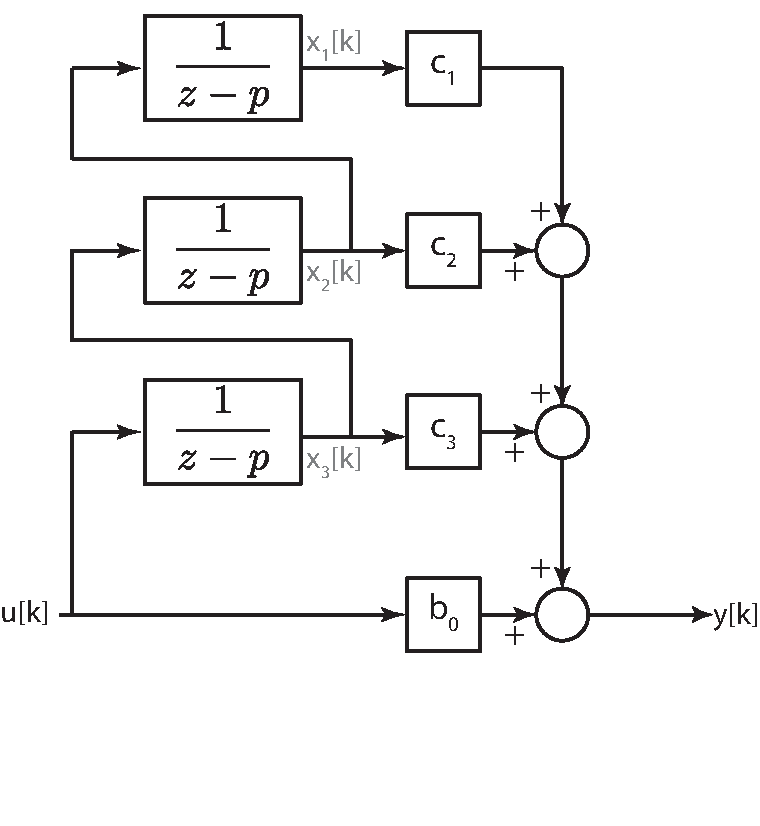
\includegraphics[width=\textwidth]{jordan}
     \end{center}
 \end{minipage}
     \end{center}
%
Now let's concentrate on the candidate ``state variables''
and try to write state evaluation equations
%
\begin{align*}
X_1(z) &= \frac{1}{z - p} X_2(z) \quad \rightarrow \quad x_1[k+1] = p \
  x_1[k] + x_2[k]
\\
X_2(z) &= \frac{1}{z - p} X_3(z) \quad \rightarrow \quad x_2[k+1] = p
         \ x_2[k] +
  x_3[k]
\\
X_3(z) &= \frac{1}{z - p} U(z) \quad \rightarrow \quad x_3[k+1] = p \
  x_3[k] + u[k]
\end{align*}
%
where as output equation can be derived as
%
\begin{align*}
y[k] &= b_0 u[k] + c_1 x_1[k] + c_2 x_2[k] + c_3 x_3[k]
\end{align*}
%
If we combine the state and output equations, we
can obtain the state space form as
%
\begin{align*}
  \mathbf{x}[k+1] &= \left[ \begin{array}{ccc} p & 1 & 0\\ 0 & p & 1
    \\ 0 & 0 & p \end{array} \right] \mathbf{x}[k]
   + 
  \left[ \begin{array}{c} 0 \\ 0
    \\ 1 \end{array} \right] u[k]
\\
y[k] &= \left[ \begin{array}{ccc} c_1 & c_2 & c_3 \end{array} \right]
+ b_0 u[k]
\end{align*}
%
where 
%
\begin{align*}
\mathbf{x} = \left[ \begin{array}{c} x_1[k] \\ x_2[k] \\
x_1[k] \end{array} \right] \quad , \quad
A = \left[ \begin{array}{ccc} p & 1 & 0 \\ 0 & p & 1
    \\ 0 & 0 & p \end{array} \right]
\quad , \quad 
B = \left[ \begin{array}{c} 0 \\ 0
    \\ 1 \end{array} \right]
\quad , \quad
C = \left[ \begin{array}{ccc} c_1 & c_2 & c_3 \end{array} \right]
\quad , \quad
D = b_0
\end{align*}
%
$A, \ B, \ \& \ C$ forms a Jordan block. 

For a general $n^{th}$ order system a Jordan block 
with $m$ repeated roots inside a stat-space representation
in Jordan canonical form looks like
%
\begin{align*}
A &= \left[ \begin{array}{c|ccccc|c} 
\ddots & & & & & &
\\ \hline
& \bar{p} & 1 & \cdots & 0 & 0 & 
\\ & 0 & \bar{p} & \cdots & 0 & 0
\\ & & & \ddots & & & 
\\ & 0 & 0 & \cdots & \bar{p} & 1
    \\ & 0 & 0 & \cdots & 0 & \bar{p}
\\
\hline
& & & & & & \ddots
 \end{array} \right]
\quad , \quad 
B = \left[ \begin{array}{c} \vdots \\\hline 
0 \\ 0 \\ \vdots \\ 0 \\  1 \\ \hline
\vdots
\end{array} \right]
\\ C &= \left[ \begin{array}{c|ccccc|c} \cdots & 
c_1 & c_2 & \cdots &  c_{n-1} & c_n & \cdots\end{array} \right]
\end{align*}
%

\begin{exmp}
Let $G(s) = \frac{s^2 + 8 s + 10}{s^2 + 3 s + 2}$
\end{exmp}
%
find a controllable, observable, and  diagonal canonical state-space representation of the given TF.

\vspace{6pt}

\textbf{Solution:}

If we follow the derivation of controllable canonical form for a
second order system we obtain the following structure
%
\begin{align*}
	\dot{x} &= \left[ \begin{array}{cc} 0 & 1  \\  -a_0 & -a_1 \end{array} \right] x 
	+ \left[ \begin{array}{c} 0 \\ 1 \end{array} \right] u
	\\
	y &= \left[ \begin{array}{ccc} ( b_0 - b_2 a_0 ) & ( b_1 - b_2
                                                           a_1 )  \end{array} \right] x
	+ \left[ b_2 \right] u
\end{align*}
%
where 
%
\begin{align*}
a_0= 2 \ , \ a_1 = 3 \ , \ b_0 = 10 \ , \ b_1 = 8 \ ,\& \ b_2 = 1
\end{align*}
%
Thus, the state-space representation takes the form
%
\begin{align*}
	\dot{x} &= \left[ \begin{array}{cc} 0 & 1  \\  -2 & -3 \end{array} \right] x 
	+ \left[ \begin{array}{c} 0 \\ 1 \end{array} \right] u
	\\
	y &= \left[ \begin{array}{ccc} 8 & 5  \end{array} \right] x + [1] u
\end{align*}
%
Observable canonical form is the dual of the controllable canonical form
thus for the given system, we know that
%
\begin{align*}
	A_{OCF} &= A_{CCF}^T = \left[ \begin{array}{cc} 0 & -2  \\  1 & -3 \end{array} \right]
		\\
	B_{OCF} &= C_{CCF}^T = \left[ \begin{array}{c} 8  \\  5 \end{array} \right]
		\\
	C_{OCF} &= B_{CCF}^T = \left[ \begin{array}{cc} 0  &  1 \end{array} \right]
	\\
	 D_{OCF} &= D_{CCF} = [1]
\end{align*}
%
In order to find the diagonal canonical form, we need to perform partial fraction
expansion 
%
\begin{align*}
G(s) &= \frac{s^2 + 8 s + 10}{s^2 + 3 s + 2}
	= 1 + \frac{3}{s+1} + \frac{2}{s+2}
\end{align*}
%
then SS matrices for the diagonal canonical form can be simply derived as
%
\begin{align*}
	A_{DCF} &=  \left[ \begin{array}{cc} -1 & 0  \\  0 & -2 \end{array} \right]
		\\
	B_{DCF} &=  \left[ \begin{array}{c} 1  \\  1 \end{array} \right]
		\\
	C_{DCF} &= \left[ \begin{array}{cc} 3  &  2 \end{array} \right]
	\\
	 D_{DCF} &=  [1]
\end{align*}

\begin{exmp}
Consider the following general state-space representation
\end{exmp} 
%
\begin{align*}
  \dot{x}(t) &= A x(t) + B u(t) , \\
  y(t) &= C x(t) + D u(t) 
\end{align*}
%
Now let's consider the following
state-space representation
%
\begin{align*}
  \dot{\bar{x}}(t) &= A^T \bar{x}(t) + C^T u(t) , \\
  y(t) &= B^T \bar{x}(t) + D u(t) 
\end{align*}
%
Show that these two state-space representations 
results in same transfer function form

\vspace{6pt}

\textbf{Solution:} 
%
For the second representation we have 
%
\begin{align*}
\bar{G}(s) &= \bar{C} \left( s I - \bar{A} \right)^{-1} \bar{B} + D
	\\
	&= B^T \left( s I - A^T \right)^{-1} C^T + D
\end{align*}
%
Since $\bar{G}(s)$ is a scalar quantity we can take its
transpose 
%
\begin{align*}
	\bar{G}(s) &= [\bar{G}(s)]^T = 
	[ B^T \left( s I - A^T \right)^{-1} C^T + D ]^T
	\\
	&= (C^T)^T \left( \left( s I - A^T \right)^{-1} \right)^T (B^T)^T + D
	\\
	&= C \left( \left( s I - A^T \right)^T \right)^{-1} B + D
	\\
	&= C \left( s I - A \right)^{-1} B + D
	\\
	\bar{G}(s) &= G(s)
\end{align*}
%
This result also shows that controllable and observable 
canonical representations are similar. 

\subsection{Canonical State-Space Realizations of SIMO Systems}

For the sake of clarity, we will only consider double output systems, however generalization to higher dimensional outputs is straightforward. 

\subsubsection{CT Reachable/Controllable Canonical Form}

\textbf{Case I:} Let transfer function matrix of a SIMO system be 
%
\begin{align*}
	G(s) = \left[ \begin{array}{c} G_1(s) \\ G_2(s) \end{array} \right] =
	       \left[ \begin{array}{cc} d_{1} + \frac{ b_{1,2} s^2  + b_{1,1} s + b_{1,0} }{ s^3 + a_2 s^2 + a_1 s + a_0}  
	       \\ d_{2} + \frac{ b_{2,2} s^2  + b_{2,1} s + b_{2,0} }{ s^3 + a_2 s^2 + a_1 s + a_0}   \end{array} \right]
\end{align*}
%
We can first obtain the $D$ matrix as
%
\begin{align*}
	D = \lim_{s \to \infty} G(s) = \left[ \begin{array}{c} d_1 \\  d_2 \end{array} \right]
\end{align*}
%
Now we concentrate the strictly proper parts of the transfer function matrix. 
Similar to SISO case we can organize the transfer function matrix equations as
%
\begin{align*}
Y(s) &=  \left[ \begin{array}{cc} b_{1,2} s^2  + b_{1,1} s + b_{1,0} 
	       \\  b_{2,2} s^2  + b_{2,1} s + b_{2,0}   \end{array} \right]
\frac{1}{ s^3 + a_2 s^2 + a_1 s + a_0 } U(s) 
= \left[ \begin{array}{c} n_1(s) \\ n_2(s) \end{array} \right] G_s(s) U(s) \ \mathrm{where} 
\\
Y(s) &= \left[ \begin{array}{c} n_1(s) \\ n_2(s) \end{array} \right] H(s) 
\\
G_s(s) &= \frac{H(s)}{U(s)} 
\end{align*}
%
$G_s(s) = \frac{H(s)}{U(s)} $ defines a SISO system and we already know its state-update equation in controllable canonical form
%
\begin{align*}
\dot{x} &= A x + B u \ , \ \mathrm{where} \ x = \left[ \begin{array}{c} h \\ \dot{h} \\ \ddot{h} \end{array} \right]
\\
A &= \left[ \begin{array}{ccc} 0 & 1 & 0  \\ 0 & 0 & 1 \\
 -a_0 & -a_1 & -a_2  \end{array} \right]
\quad , \quad 
B = \left[ \begin{array}{c} 0 \\ 0 \\  1 \end{array} \right]
\end{align*}
%
Not let's focus on $Y(s) = \left[ \begin{array}{c} N_1(s) \\ N_2(s) \end{array} \right] H(s) $ and take its inverse Laplace transform
%
\begin{align}
  y &= \left[ \begin{array}{c} b_{1,2} \ddot{h}  + b_{1,1} \dot{h} + b_{1,0} h
	       \\  b_{2,2} \ddot{h} + b_{2,1} \dot{h} + b_{2,0}  h \end{array} \right] = \left[ \begin{array}{ccc} b_{1,0}  & b_{1,1}  & b_{1,2} 
	       \\  b_{2,0}  &  b_{2,1} & b_{2,2}  \end{array} \right] x
	       \\
	       C &= \left[ \begin{array}{ccc} b_{1,0}  & b_{1,1}  & b_{1,2} 
	       \\  b_{2,0}  &  b_{2,1} & b_{2,2}  \end{array} \right]
\end{align}
% 
It is quite straightforward to extend this operation to higher orders

\textbf{Case II:} Now consider a case where the transfer function matrix of a SIMO system has the following form
%
\begin{align*}
	G(s) = \left[ \begin{array}{c} G_1(s) \\ G_2(s) \end{array} \right] = \left[ \begin{array}{c} \frac{n_1(s)}{d_1(s)} \\ \frac{n_2(s)}{d_2(s)} \end{array} \right]	      
	\ , \ \mathrm{where} \ d_1(s) \neq d_2(s)
\end{align*}
% 
Obviously we can not directly apply the standard approach for this problem. In this case, one first finds
the \textit{monic least common denominator} of all entries of the transfer function matrix (i.e. the least common multiple of the
denominators of all the entries), $d_c(s)$ then we re-write the transfer function matrix as
%
\begin{align*}
	G(s) = \left[ \begin{array}{c} G_1(s) \\ G_2(s) \end{array} \right] = \left[ \begin{array}{c} \frac{n_1(s)}{d_1(s)} \\ \frac{n_2(s)}{d_2(s)} \end{array} \right]	      
	= \left[ \begin{array}{c} \frac{n_1(s) d_c(s) / d_1(s) }{d_c(s)} \\ \frac{n_2(s) d_c(s) / d_2(s)}{d_c(s)} \end{array} \right]	      
\end{align*}
% 
and realize the transfer function using the controllable canonical form
 
\subsection{Canonical State-Space Realizations of MISO Systems}

For the sake of clarity, we will only consider double output systems, however generalization to higher dimensional outputs is straightforward. 

\subsubsection{DT Observable Canonical Form}

\textbf{Case I:} Let transfer function matrix of a MISO system be 
%
\begin{align*}
	G(z) = \left[ \begin{array}{cc} G_1(z) & G_2(z) \end{array} \right] =
	\left[ \begin{array}{cc} 
	d_{1} + \frac{ b_{1,2} z^{-1} + b_{1,1} z^{-2} + b_{1,0} z^{-3} }{ 1 + a_2 z^{-1} + a_1 z^{-2} + a_0 z^{-3} }  
	& 
	d_{2} + \frac{ b_{2,2} z^{-1} + b_{2,1} z^{-2} + b_{2,0} z^{-3} }{ 1 + a_2  z^{-1} + a_1 z^{-2} + a_0 z^{-3}  } 
	\end{array} \right]
\end{align*}
%
We can first obtain the $D$ matrix as
%
\begin{align*}
	D = \lim_{z \to \infty} G(z) = \left[ \begin{array}{cc} d_1 &  d_2 \end{array} \right]
\end{align*}
%
Now we concentrate the strictly proper parts of the transfer function matrix. 
Let's start with the frequency domain expression of the single output 
and perform some grouping based on the delay elements.
%
{\small
\begin{align*}
&Y(z) ( 1+ a_2 z^{-1} + a_1 z^{-2} + a_0 z^{-3} ) 
= ( b_{1,2} z^{-1} + b_{1,1} z^{-2} + b_{1,0} z^{-3} ) U_1(z) 
+ ( b_{2,2} z^{-1} + b_{2,1} z^{-2} + b_{2,0} z^{-3} ) U_2(z) 
\\
&Y(z) = z^{-1} \left(  b_{1,2} U_1(z) + b_{2,2} U_2(z) - a_2 Y(z) \right) + z^{-2} \left( b_{1,1} U_1(z) + b_{2,1} U_2(z)  -
  a_1 Y(z) \right) 
  \\ & \quad \quad \quad + z^{-3} \left( b_{1,0} U_1(z) + b_{2,0} U_2(z)  - a_0 Y(z) \right)
\\
&= \frac{1}{z} \left\lbrace \left( b_{1,2} U_1(z) + b_{2,2} U_2(z) - a_2 Y(z) \right) + \frac{1}{z} \left[ \left( b_{1,1} U_1(z) + b_{2,1} U_2(z) -
  a_1 Y(z) \right) + \frac{1}{z} \left( b_{1,0} U_1(z) + b_{2,0} U_2(z)  - a_0 Y(z) \right) \right] \right\rbrace 
\end{align*}
}
%
As you can see we have only $z^{-1}$ terms in the representation there
is a special topology embedded inside the expression. Let the
Z-transform domain representations of state variables 
$X(z) = \left[ \begin{array}{c} X_1(z) \\ X_2(z) \\ X_3(z) \end{array} \right]$ defined as 
%
\begin{align*}
X_1(z) &= \frac{1}{z} \left( -a_0 X_3(z) + b_{1,0} U_1(z) + b_{2,0} U_2(z) \right)
\\
X_2(z) &= \frac{1}{z}  \left\lbrace \left( -a_1 X_3(z) + b_{1,1} U_1(z) + b_{2,1} U_2(z) \right) + 
X_1(z) \right\rbrace
\\
X_3(z) &= \frac{1}{z} \left[ \left( -a_2 X_3(z) + b_{1,2} U_1(z) + b_{2,2} U_2(z) \right) + X_2(z) \right]
\end{align*}
%
In this context output equation in $z$ and time domains simply takes the form
%
\begin{align*}
	Y(z) = X_3(z) + D \left[ \begin{array}{c} U_1(z) \\  U_2(z) \end{array} \right] \quad \rightarrow \quad 
	y[k] = \left[ \begin{array}{ccc} 0 & 0 & 1 \end{array} \right] x[k] + D \left[ \begin{array}{c} u_1[k] \\  u_2[k] \end{array} \right] 
\end{align*}
% 
State equations (in $z$ and time domains) take the form
%
%
{\small
\begin{align*}
z X_1(z) = -a_0 X_3(z)  + b_{1,0} U_1(z) + b_{2,0} U_2(z) \, &\rightarrow \, x_1[k+1] = -a_0 x_3[k]  + b_{1,0} u_1[k] + b_{2,0} u_2[k] 
\\
z X_2(z) = X_1(z)  - a_1 X_3(z) + b_{1,1} U_1(z) + b_{2,1} U_2(z) U(z)  \, &\rightarrow \, x_2[k+1] = x_1[k]  - a_1 x_3[k] + b_{1,1} u_1[k] + b_{2,1} u_2[k] 
\\
z X_3(z) = X_2(z)  - a_2 X_3(z) + b_{1,2} U_1(z) + b_{2,2} U_2(z) U(z)  \, &\rightarrow \, x_3[k+1] = x_2[k]  - a_2 x_3[k] + b_{1,2} u_1[k] + b_{2,2} u_2[k] 
\end{align*}
}
%
If we re-write all equations in matrix form, we obtain the state-space representation as
%
\begin{align*}
	x[k+1] &= \left[ \begin{array}{ccc} 0 & 0 & -a_0  \\  1 & 0 & -a_1 \\  0 & 1 & -a_2 \end{array} \right] x[k] 
	+ \left[ \begin{array}{cc} b_{1,0} &  b_{2,0} \\ b_{1,1} &  b_{2,1} \\ b_{1,2} &  b_{2,2} \end{array} \right] u[k]
	\\
	y[k] &= \left[ \begin{array}{ccc} 0 & 0  & 1 \end{array} \right] x[k]
	+ \left[ \begin{array}{cc} d_1 &  d_2 \end{array} \right] u[k]
\end{align*}
%
It is quite straightforward to extend this operation to higher orders. Note that for MISO systems
with $d_1(s) \neq d_2(s)$ where $G_1(s) = \frac{n_1(s)}{d_1(s)}$ and $G_2(s) = \frac{n_2(s)}{d_2(s)}$
we can not directly apply same operations. However similar to the controllable canonical form in SIMO systems
we can start by finding the \textit{monic least common denominator} of all entries of the transfer function matrix (i.e. the least common multiple of the
denominators of all the entries), $d_c(s)$ then we re-write the transfer function using the similar format in controllable 
canonical form. After that we can apply the MISO observable canonical form derivations to realize the state-space structure. 

\subsection{Canonical State-Space Realizations of MIMO Systems} 

\subsubsection{Gilbert's Realization - MIMO Generalization of Diagonal Canonical Form}

Suppose we have a transfer function matrix $G(s) \in \mathbb{T}^{q \times p}$ (where $\mathbb{T}$ is the vector space of all proper transfer functions).
First find/compute the least common denominator, $d_c(s)$,  of all the entries of $G(s)$. If $d_c(s)$ has no repeated 
poles, then we can find a \textit{minimal} state-space realization in the form of generalized diagonal canonical form 
using Gilbert's method. Now, a partial fraction expansion to each of the elements of  $G(s)$ and collect residue matrices, $R_i \in \mathbb{C}^{q \times p}$ for
each distinct pole. Not we can re-write the transfer function matrix in the following form
%
\begin{align*}
G(s) = D + \sum_{i=1}^{N_p} R_i \frac{1}{(s - \rho_i)} 
\end{align*}
%
where $D = \lim_{s \to \infty} G(s)$, $\rho_i$'s denotes the $N_p$ distinct poles/roots, and $R_i \in \mathbb{C}^{q \times p}$ denotes the residue matrix 
for each $\rho_i$. Let $r_i = \mathrm{Rank}(R_i)$, then $r_i$ gives the number of poles required the mode associated with $\rho_i$. We know that (from Linear Algebra) we can write $R_i$ in terms of multiplication of two full rank matrices
%
\begin{align*}
R_i = C_i  B_i , \ \mathrm{where} \ C_i \in \mathbb{C}^{q \times r_i} \ ,  \ B_i \in \mathbb{C}^{r_i \times p}  
\end{align*}
%
then each state-equation associated with mode $\rho_i$ takes the form
%
\begin{align*}
\dot{x}_i &= \left[ \begin{array}{cccc} \rho_i & 0 & \cdots & 0 \\  0 & \ddots & & \vdots \\  \vdots  & & \ddots & 
\\  0  & \cdots & 0 & \rho_i \end{array} \right] x_i
	+ B_i u \ , \ x_i \in \mathbb{R}^{r_i} \ , \ u \in \mathbb{R}^{q}
	\\
	y &= C_i x_i 
\end{align*}
%
whole state-space structure will be in diagonal canonical form 
%
\begin{align*}
\dot{x} &= \left[ \begin{array}{cccc} A_1 & 0 & \cdots & 0 \\  0 & \ddots & & \vdots \\  \vdots  & & \ddots & 
\\  0  & \cdots & 0 & A_{N_P} \end{array} \right] x + 
\left[ \begin{array}{c} B_1 \\ \vdots \\ B_{N_P} \end{array} \right] u \ , \ x = \left[ \begin{array}{c} x_i \\ \vdots \\ x_{N_P} \end{array} \right]
\\
y &= \left[ \begin{array}{ccc} C_1 & \cdots & C_{N_P} \end{array} \right] x + D 
\end{align*}
%

\begin{exmp}
Let %
\begin{align*}
	G(s) = \left[ \begin{array}{c} G_1(s) \\ G_2(s) \end{array} \right] = 
	       \left[ \begin{array}{cc} \frac{ 1 }{ s^2 + s }  
	       \\ \frac{ 1 }{ s }   \end{array} \right] =  \left[ \begin{array}{cc} \frac{ 1 }{ s }  - \frac{ 1 }{ s + 1 } 
	       \\ \frac{ 1 }{ s }  \end{array} \right] 
\end{align*}
%  
\end{exmp}
%
Find reachable and diagonal canonical (both minimal) state-space representations of the given SIMO system

\textbf{Solution:} Let's start with reachable canonical realization. For the given system $d_c(s) = s(s+1)$ and hence we can re-write the 
transfer function matrix as
%
\begin{align*}
	G(s) =  \left[ \begin{array}{cc} \frac{ 1 }{ s^2 + s }  
	       \\ \frac{ s+1 }{ s^2 + s}   \end{array} \right] 
\end{align*}
%  
If we follow the reachable canonical forms derivation for SIMO systems we can obtain
%
%
\begin{align*}
A &= \left[ \begin{array}{ccc} 0 & 1 \\ 0 & -1  \end{array} \right]
\quad , \quad 
B = \left[ \begin{array}{c} 0 \\  1 \end{array} \right]
\quad , \quad 
	C = \left[ \begin{array}{cc} 1  & 0
	       \\  1  &  1  \end{array} \right]
\end{align*}
% 
Now let's find the diagonal canonical form using Gilbert's method
\begin{align*}
	&G(s) =  \left[ \begin{array}{cc} \frac{ 1 }{ s }  - \frac{ 1 }{ s + 1 } 
	       \\ \frac{ 1 }{ s }  \end{array} \right]  = \left[ \begin{array}{cc} \frac{ -1 }{ s + 1 } 
	       \\ 0  \end{array} \right]  + \left[ \begin{array}{cc} \frac{ 1 }{ s }  
	       \\ \frac{ 1 }{ s }  \end{array} \right] = \left[ \begin{array}{cc} -1
	       \\ 0  \end{array} \right] \frac{ 1 }{ s + 1 }  + \left[ \begin{array}{cc} 1
	       \\ 1  \end{array} \right] \frac{ 1 }{ s }  
	     \\
	  &   \rho_1 = -1 \ , \ R_1 = \left[ \begin{array}{cc} -1
	       \\ 0  \end{array} \right] = C_1 B_1 = \left[ \begin{array}{cc} -1
	       \\ 0  \end{array} \right] [1]
	       \\
	       	  &   \rho_2 = 0 \ , \ R_2 = \left[ \begin{array}{cc} 1
	       \\ 1  \end{array} \right] = C_2 B_2 = \left[ \begin{array}{cc} 1
	       \\ 1  \end{array} \right] [1]
\end{align*}
%
We can than find the state-space matrices 
%
\begin{align*}
A &= \left[ \begin{array}{ccc} -1 & 0 \\ 0 & 0  \end{array} \right]
\quad , \quad 
B = \left[ \begin{array}{c} 1 \\  1 \end{array} \right]
\quad , \quad 
	C = \left[ \begin{array}{cc} -1  & 1
	       \\  0 &  1  \end{array} \right]
\end{align*}
% 

\begin{exmp}
Let %
\begin{align*}
	G(s) = \left[ \begin{array}{cc} G_1(s) & G_2(s) \end{array} \right] = 
	       \left[ \begin{array}{cc} \frac{ 1 }{ s^2 + s }  &
	        \frac{ 1 }{ s }   \end{array} \right] =  \left[ \begin{array}{cc} \left( \frac{ 1 }{ s }  - \frac{ 1 }{ s + 1 } \right) &
	        \frac{ 1 }{ s }  \end{array} \right] 
\end{align*}
%  
\end{exmp}
%
Find observable and diagonal canonical (both minimal) state-space representations of the given MISO system

\textbf{Solution:} Let's start with observable canonical realization. For the given system $d_c(s) = s(s+1)$ and hence we can re-write the 
transfer function matrix as
%
\begin{align*}
	G(s) =  \left[ \begin{array}{cc} \frac{ 1 }{ s^2 + s }  
	       &  \frac{ s+1 }{ s^2 + s}   \end{array} \right] 
\end{align*}
%  
If we follow the reachable canonical forms derivation for MISO systems we can obtain
%
%
\begin{align*}
A &= \left[ \begin{array}{ccc} 0 & 0 \\ 1 & -1  \end{array} \right]
\quad , \quad 
B = \left[ \begin{array}{cc} 1 & 1 \\  0 & 1 \end{array} \right]
\quad , \quad 
	C = \left[ \begin{array}{cc} 0  & 1  \end{array} \right]
\end{align*}
% 
Now let's find the diagonal canonical form using Gilbert's method
\begin{align*}
	G(s) &=  \left[ \begin{array}{cc} \frac{ 1 }{ s }  - \frac{ 1 }{ s + 1 }  &  \frac{ 1 }{ s }  \end{array} \right]  = 
	\left[ \begin{array}{cc} \frac{ -1 }{ s + 1 }  & 0  \end{array} \right]  
	+ \left[ \begin{array}{cc} \frac{ 1 }{ s }  & \frac{ 1 }{ s }  \end{array} \right] 
	\\ &= \left[ \begin{array}{cc} -1 & 0  \end{array} \right] \frac{ 1 }{ s + 1 }  + \left[ \begin{array}{cc} 1 & 1  \end{array} \right] \frac{ 1 }{ s }  
	     \\
	    \rho_1 & = -1 \ , \ R_1 = \left[ \begin{array}{cc} -1
	       & 0  \end{array} \right] = C_1 B_1 = [1] \left[ \begin{array}{cc} -1
	       & 0  \end{array} \right] 
	       \\
	       	     \rho_2 & = 0 \ , \ R_2 = \left[ \begin{array}{cc} 1
	       & 1  \end{array} \right] = C_2 B_2 = [1] \left[ \begin{array}{cc} 1
	       & 1  \end{array} \right] 
\end{align*}
%
We can than find the state-space matrices 
%
\begin{align*}
A &= \left[ \begin{array}{ccc} -1 & 0 \\ 0 & 0  \end{array} \right]
\quad , \quad 
B = \left[ \begin{array}{cc} -1 & 0 \\  1 & 1 \end{array} \right]
\quad , \quad 
	C = \left[ \begin{array}{cc} 1  & 1  \end{array} \right]
\end{align*}
% 

\begin{exmp}
Let %
\begin{align*}
	G(s) = \left[ \begin{array}{cc} G_{11}(s) & G_{12}(s) \\ G_{21}(s) & G_{22}(s) \end{array} \right]  =  \left[ \begin{array}{cc} \left( \frac{ 1 }{ s }  - \frac{ 1 }{ s + 1 } \right) &
	        \frac{ 1 }{ s }  \\ 	\frac{ 1 }{ s } & 0  \end{array} \right] 
\end{align*}
%  
\end{exmp}
%
Find a diagonal canonical (minimal) state-space representations of the given MIMO system.

\textbf{Solution:} For the given system $d_c(s) = s(s+1)$. let's find the diagonal canonical form using Gilbert's method
\begin{align*}
	G(s) &= \left[ \begin{array}{cc} \left( \frac{ 1 }{ s }  - \frac{ 1 }{ s + 1 } \right) &
	        \frac{ 1 }{ s }  \\ 	\frac{ 1 }{ s } & 0  \end{array} \right]   = 
	\left[ \begin{array}{cc} \frac{ -1 }{ s + 1 }  & 0 \\ 0 & 0 \end{array} \right]  
	+ \left[ \begin{array}{cc} \frac{ 1 }{ s }  & \frac{ 1 }{ s } \\ \frac{ 1 }{ s } & 0 \end{array} \right] 
	\\ &= \left[ \begin{array}{cc} -1 & 0 \\ 0 & 0  \end{array} \right] \frac{ 1 }{ s + 1 }  + \left[ \begin{array}{cc} 1 & 1 \\ 1 & 0 \end{array} \right] \frac{ 1 }{ s }  
	     \\
	    \rho_1 & = -1 \ , \ R_1 = \left[ \begin{array}{cc} -1
	       & 0 \\ 0 & 0  \end{array} \right] = C_1 B_1 = \left[ \begin{array}{c} 1 \\ 0  \end{array} \right] \left[ \begin{array}{cc} -1 
	       & 0  \end{array} \right] \ , \ \mathrm{Rank}(R_1) = 1
	       \\
	       	     \rho_2 & = 0 \ , \ R_2 = \left[ \begin{array}{cc} 1
	       & 1  \\ 1 & 0 \end{array} \right] = C_2 B_2 = \left[ \begin{array}{cc} 1
	       & 1  \\ 1 & 0 \end{array} \right] \left[ \begin{array}{cc} 1
	       & 0 \\ 0 & 1  \end{array} \right] \ , \ \mathrm{Rank}(R_2) = 2
\end{align*}
%
We can than find the state-space matrices 
%
\begin{align*}
A &= \left[ \begin{array}{c|cc} -1 & 0 & 0 \\ \hline 0 & 0 & 0 \\ 0 & 0 & 0   \end{array} \right]
\quad , \quad 
B = \left[ \begin{array}{cc} -1 & 0 \\  \hline 1 & 0 \\ 0 & 1 \end{array} \right]
\quad , \quad 
	C = \left[ \begin{array}{c|cc} 1  & 1 & 1 \\ 0 & 1 & 0  \end{array} \right]
\end{align*}
% 

\newpage

\section{Equivalent State-Space Representations}

\textbf{Definition:} If two different quadruples $(A , B , C , D)$ and $(\bar{A} , \bar{B} , \bar{C} , \bar{D})$ yield the same transfer function matrix, 
i.e. $C (z I - A)^{-1} B + D = \bar{C} (z I - \bar{A})^{-1} \bar{B} + \bar{D}$, then the systems
%
\begin{align*}
 \left\lbrace x[k+1] = A x[k] + B u[k] \ , \  y[k] = C x[k] + D u[k] \right\rbrace \&  \left\lbrace \bar{x}[k+1] = \bar{A} \bar{x}[k] + \bar{B} u[k] \ , \  y[k] = \bar{C} \bar{x}[k] + \bar{D} u[k] \right\rbrace
\end{align*}
are said to be \textit{zero-state-equivalent} (ZSE).

Note that if two systems are ZSE, under zero-initial conditions, they give the same output response when excited by the same input (for all inputs).

\textbf{Definition:} Consider the n-dimensional LTI system
%
\begin{align*}
  x[k+1] = A x[k] + B u[k] \ , \  y[k] = C x[k] + D u[k] \ (S_1)
\end{align*}
%
The LTI system given as 
%
\begin{align*}
  \hat{x}[k+1] = \hat{A} \hat{x}[k] + \hat{B} u[k] \ , \  y[k] = \hat{C} \hat{x}[k] + \hat{D} u[k] \ (S_2)
\end{align*}
%
is said to be \textit{algebraically equivalent} (AE) to $S_1$ if $D = \hat{D}$ and  $\exists P \in \mathbb{C}^{n \times n} \quad \mathrm{det}(P) \neq 0$
that satisfies $\hat{A} = P  A P^{-1} \ , \ \hat{B} = P B \ , \ \hat{C} = C P $.

\textbf{Remark:} $S_2$ corresponds to the state vector transformation $ P x[k] = \hat{x}[k]$
%
\begin{align*}
  P^{-1} \hat{x}[k+1] = A P^{-1} \hat{x}[k] + B u[k] 
\quad &, \quad y[k] = C P^{-1} \hat{x}[k] + D u[k]
\\
  \hat{x}[k+1] = P A P^{-1} \hat{x}[k] + P B u[k] 
\quad &, \quad y[k] = C P^{-1} \hat{x}[k] + D u[k]
\end{align*}
%
where
%
\begin{align*}
\hat{A} &= P  A P^{-1} \ , \ \hat{B} = P  B \ , \ \hat{C} = C P^{-1} \ ,   \ \hat{D} = D
\end{align*}
%
Since there exist infinitely many non-singular $n \times n$
matrices, for a given LTI system, there exist infinitely 
many different but AE  state-space representations.

\vspace{12pt}

\begin{exmp}
Show that $A \in \mathbb{R}^{n \times n}$ and $P^{-1} A P$, where $P \in \mathbb{R}^{n \times n}$ and $\mathrm{det}(P) \neq 0$, have the same characteristic equation
\end{exmp}

\textbf{Solution:} 
\begin{align*}
  \mathrm{det}\left(\lambda I - P^{-1} A P \right) &= 
\mathrm{det}\left( \lambda P^{-1} I P - P^{-1} A P \right)
\\
&= \mathrm{det} \left( P^{-1} \left( \lambda I - A \right) P \right)
\\
&= \mathrm{det} \left( P^{-1} \right)
\mathrm{det} \left( \lambda I - A \right) 
\mathrm{det} \left( P \right)
\\
&= \mathrm{det} \left( P^{-1} \right) \mathrm{det} \left( P \right)
\mathrm{det} \left( \lambda I - A \right) 
\\
\mathrm{det}\left(\lambda I - P^{-1} A P \right) &= \mathrm{det} \left( \lambda I - A \right) 
\end{align*}

\textbf{Theorem:} Algebraically equivalent systems has the same transfer function matrix

Consider the two different AE state-space representations
%
\begin{align*}
  x[k+1] = A x[k] + B u[k]  \quad & \quad \quad \hat{x}[k+1] = \hat{A} \hat{x}[k] + \hat{B} u[k] 
\\
  y[k] = C x[k] + D u[k] \quad & \quad \quad  y[k] = \hat{C} x[k] + \hat{D} u[k]
\end{align*}
%
where they are related with the following similarity transformation
%
\begin{align*}
P x[k] = \hat{x}[k] \ , \
\hat{G} &= P  G P^{-1} \ , \ \hat{H} = P  H \ , \ \hat{C} = C P^{-1} \ ,
  \ \hat{D} = D
\end{align*}
%
Let's compute the transfer function for the second representation
%
\begin{align*}
  \hat{T}(z) &= \left[ \hat{C} \left(z I - \hat{G} \right)^{-1} \hat{H}
  + \hat{D} \right]
\\
&= \left[ C P^{-1} \left(z I - P  G P^{-1} \right)^{-1} P H
  + D \right]
\\
&= \left[ C P^{-1} \left( P \left( z I -   G \right) P^{-1} \right)^{-1} P H
  + D \right]
\\
&= \left[ C P^{-1} P \left( z I -   G \right)^{-1} P^{-1} P H
  + D \right]
\\
&= \left[ C \left( z I -   G \right)^{-1} H + D \right]
\\
\hat{T}(z) &= T(z)
\end{align*}


\end{document}
